% Chapter Template

\chapter{Control} % Main chapter title

\label{Chapter 2} % Change X to a consecutive number; for referencing this chapter elsewhere, use \ref{ChapterX}

\lhead{Chapter 2. \emph{Control}} % Change X to a consecutive number; this is for the header on each page - perhaps a shortened title

%
Once the simulation is fully implemented, the goal is to use it as a testbench for different ways of controlling the structure. The second part of the project will be fully consecrated on this part. A few tools have been implemented to test some of the algorithms that are used in such problems. 

\section{PID Control of the joints}

One of the problem to control accurately a joint is to adapt the command so that it can adapt to difficult situation. For instance, it is easier to walk in a swimmingpool than on the ground and this is why people recovering after an injury do aquatic training. For a joint, it can be easy to do a movement in the air, but the same movement is more difficult when touching the ground. One way to avoid this problem is to implement PID (Proportional Integral Derivative) controller. This kind of controller is used in a lot of different situation in the world of automation to control degrees of freedom. In or case, servomotors often integrate such loops to account for these changes of use. In the simulation, at each step, the command of each degree of freedom of the structure is calculated using such a PID controller. 


\begin{figure}[htbp]
    \centering
    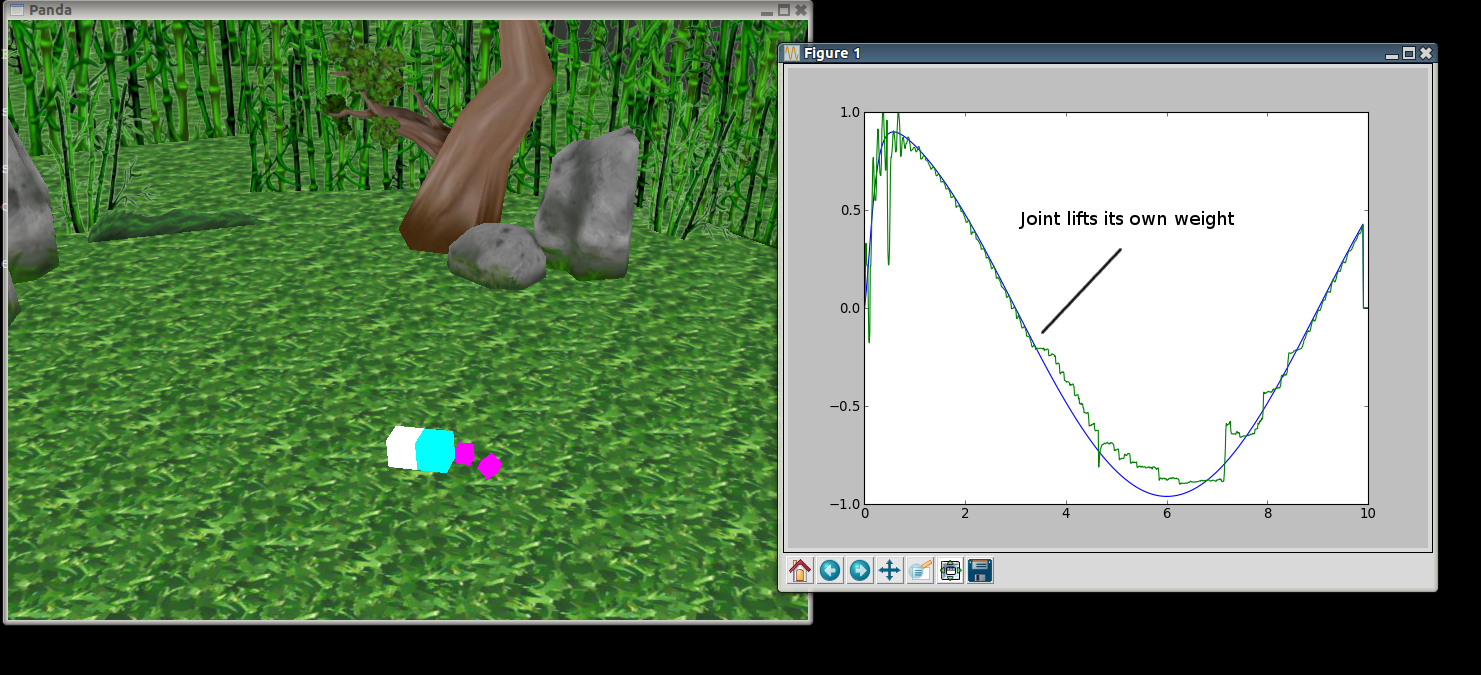
\includegraphics[scale=0.3]{Figures/servomotor.png}
    \rule{35em}{0.5pt}
    \caption[Answer of a joint to a sinusoid command]{Answer of the joint to a sinusoid command with PID Control}
    \label{fig:Snake}
\end{figure}


A few issues come from introducing PID in this problem. The stability is one of them. The PID loops need to be fast enough to be stable, which means that reducing the time between two steps of calculation on the physical world. The other problem is more a biological concern. The main goal of this project is to find solutions that are biologically inspired instead of using a classical automation approach. Therefore though the use of PID is necessary in many robotics applications, we will try to avoid using them in generating oscillations. 

\section{Central Pattern Generator}

Central Pattern Generators (CPGs) are neural networks, that can generate oscillation for the control of the muscles of or body. They are the consequence and the cause of the paradigm of periodic movement in the locomation of animals. Different models have been implemented to represent CPGs. We can represent them as a graph of coupled oscillator, where each node influence the behavior of its neighbours. For a first implementation I choose to test the model of CPG followed at EPFL ( ## INCLUDE CITATION ##). The CPG Neural Network in that case, is a graph that follow the physical architecture of the robot, settting one node for each joint (hinge or vertebra) on the structure. The dynamic of the CPG is determined by a coupling weight matrix $w_{ij}$ a phase bias matrix between nodes $\varphi_{ij}$, setting the frequency of the different oscillator $\omega_i$ and the desired amplitude and offset of the oscillation. We can compute the angle using the following system of equation and an integration method (I used the Runge-Kutta method in this project)

\begin{equation*}
    \dot{\phi_i} = \omega_i + \sum{w_{ij} * r_j * sin(\phi_i - \phi_j - \varphi_{ij}) \tag{1}
\end{equation*}
\begin{equation*}
        \theta_i = x_i + r_i * cos(\phi_i)  \tag{2}
\end{equation*}
This two equation gives the angle of the oscillator ($\theta_i$) depending on the state variable of a node: $x_i$, $r_i$, $\phi_i$, that can be described respectively as the offset, the amplitude and the phase of the oscillator.

\begin{equation*}
    \acute{r_i} = ar(\frac ar (R_i - r_i) - \dot{r_i}) \tag{3}
\end{equation*}
\begin{equation*}
    \acute{x_i} = ax(\frac ax (X_i - x_i) - \dot{x_i}) \tag{4}
\end{equation*}

Equations (3) and (4) describe the dynamic of the amplitude and offset (a second order dynamic that converge to the desired values). This trick is to ensure continuity in the oscillations, even if some of the parameters of the oscillator change. $a_r$ and $a_x$ are gains to control the dynamic ($a_r = a_x = 20 rad/s$ ##CITATION## ). 


A modification of this model is possible to plug the measured value of the degrees of freedom. Instead of using the second order control loop on $\theta_i$ which is achieved with the PID, we can set this control on the phase. Thatway, if the joint has troubles achieving his movement, for instance when hitting the ground, the phase will be modified and the perturbation will have an impact on othe joints through equation (1).

Oneway to do so is to add a term in the equation (1), with $\dot{\theta_{reali}}$ the mesured angle velocity of the joint. 
\begin{equation*}
    \dot{\phi_i} = \omega_i + \sum{w_{ij} * r_j * sin(\phi_i - \phi_j - \varphi_{ij}) + a_{\phi} * \frac {\dot{\theta_{reali}} - \dot{\theta_i}} {r_i * sin (\phi_i)} \tag{1}
\end{equation*}

If we derive (2) we get: 
\begin{equation*}
    \dot{\theta_i} = \dot{x_i} + \dot{r_i} * cos(\phi_i) + r_i * sin(\phi_i) * \dot{\phi_i} \tag{2'}
\end{equation*}

By making the assumption that the dynamic of the amplitude and the offset is slow compared to the phase, we get
\begin{equation*}
    \dot{\theta_i} = r_i * sin(\phi_i) * \dot{\phi_i} \tag{2''}
\end{equation*}
Thatway, if we consider small variation of the phase, we can deduce an error term on $\dot{\phi_i}$ from the error on $\dot{\theta_i}$ given by $\frac {\dot{\theta_{reali}} - \dot{\theta_i}} {r_i * sin (\phi_i)}$ that we can control with a gain ($a_{\phi}$).
For example if the movement of a joint is made difficult because of the ground, then the mesured velocity of this joint will be smaller that expected. The consequence will be to accelerate the movement for this joint (the derivative of the phase will be bigger), but also for the other joints that are linked to this one. 


\section{Learning}

It is then possible to learn the parameters of the CPG to optimize the movement of the structure. Instead of having to find the value of the angles, the CPGs act as basis function for the angles, and thatway we reduce the space of research to a space with finite dimensions. All the parameters (frequency, offset and amplitude of each node) are scaled to fit between $0$ and $1$. A simple fitness function can be extracted from the Simulation, for example the distance traveled by the head of the structure. It is not possible to get a gradient or Hessian matrix for this problem, as the function comes from the simulation. Moreover, the fitness function is not likely to be convex, as taking the mean of two good solutions for the movement of a structure does not necessary provide a good solution. The fitness function can also present some discontinuities or high variations because of collisions. Collisions are not are not continuous phenomenon and even if the physics engine use smoothing techniques to simplify interractions, there is a very small difference between a biped structure walking and a biped structure almost walking but with one leg that does not touch the ground, but the fitness function will give completely different results as one structure is moving and the other is not. Finally there is also the problem of consistency of a result, because two structures can behave differently for the same parameters, as the simulation can show chaotic behavior as small variations can have a big impact on the movement. 

\subsection{Random Search}

A first very simple way of finding good solution is random search. We test a random set of parameters and keep the vector of parameters showing the best results. This has the benefit of being very simple to implement and provides a good testbench for fixing issues with the simulation. A first problem observed was the consistency of the solution, testing the same parameters can lead to very different results. A first way to correct this was to take longer sample (about 20 sec of simulation). Even with this correction, online learning brought some issues, as it is possible that a good results is only good because of the initial configuration given by testing previous movement. A way to correct this is to set all angles to a default value and wait for the structure to be have a null velocity. This also led to some issues and showed solution using the first movement to jump as far as poissible. 
